\documentclass{beamer}
\usepackage[utf8]{inputenc}
\usepackage[ngerman]{babel}
\usepackage{lastpage}
\usepackage{eurosym}
\usepackage{tikz}
\usetikzlibrary{positioning}
\usetikzlibrary{arrows}
\usetikzlibrary{arrows.meta}

\input{flat-blue-theme.inc}
\beamertemplatenavigationsymbolsempty
\setbeamercovered{invisible}

\author[Hauke Stieler]{Hauke Stieler\\\href{mailto:4stieler@informatik.uni-hamburg.de}{4stieler@inf}}
\title{Liebe DB, ich hab da mal 'ne Frage}
\date{\today}

\begin{document}
	\maketitle
	
	\begin{frame}[plain]
		\Large
		Warum bekomme ich immer Briefe, wenn ich eine Erstattung wegen Verspätung beantrage?\pause\ Warum keine Mails?\pause\ Kann ich das irgendwo ändern?\pause\ Wie viele Briefe verschickt ihr so?\pause\ Und was kostet das?\pause \\
		\vspace{0.5cm}
		\begin{center}
			
\includegraphics[width=0.5\textheight]{images/thinking-meme}
		\end{center}
	\end{frame}
	
	\begin{frame}[plain]
		\begin{center}
			
\includegraphics[width=\textheight]{images/typing-meme}
		\end{center}
	\end{frame}

	\begin{frame}[plain]
		\begin{tikzpicture}[->,>=stealth']
			\draw[gray] (-2.5,4) -> (-1.5,4);
			\node[gray,anchor=west] at (-1.5,4) {Kommunikation};
			
			\draw[gray,dashed] (-2.5,3.5) -> (-1.5,3.5);
			\node[gray,anchor=west] at (-1.5,3.5) {Verwiesen an};
			
			\pause
			
			\node (me) at (0,0) {Ich};
			
			\pause
			
			\node (chatbot) at (4,3.5) {Chatbot\ \tiny(20.5.)};
			\draw (me) edge[<->] (chatbot);
			\pause
			
			\node (chat) at (4.5,1.75) {Chat\ \tiny(20.5.)};
			\draw[dashed] (chatbot) -> (chat);
			\pause
			
			\draw (me) edge[<->] (chat);
			\pause
			
			\node (kontakt) at (4.75,0) {Kontaktformular\ \tiny(20.5.)};
			\draw[dashed] (chat) -> (kontakt);
			\pause
			
			\draw (me) -> (kontakt);
			\pause
			
			\node (db) at (4.5,-1.75) {Kundendialog\ \tiny(27.5.)};
			\draw (kontakt) -> (db);
			\pause
			
			\draw (db) -> node[below] {\small Mail} (me);
			\pause
			
			\node (fahrgastrechte) at (4,-3.5) {Fahrgastrechte\ \tiny(25.6.)};
			\draw (db) -> (fahrgastrechte);
			\pause
			
			\draw (fahrgastrechte) -> node[below left] {\small \textbf{Brief}} (me);
		\end{tikzpicture}
	\end{frame}

	\begin{frame}[plain]
		\begin{tikzpicture}
			\node[anchor=south west,inner sep=0] at (0,0) {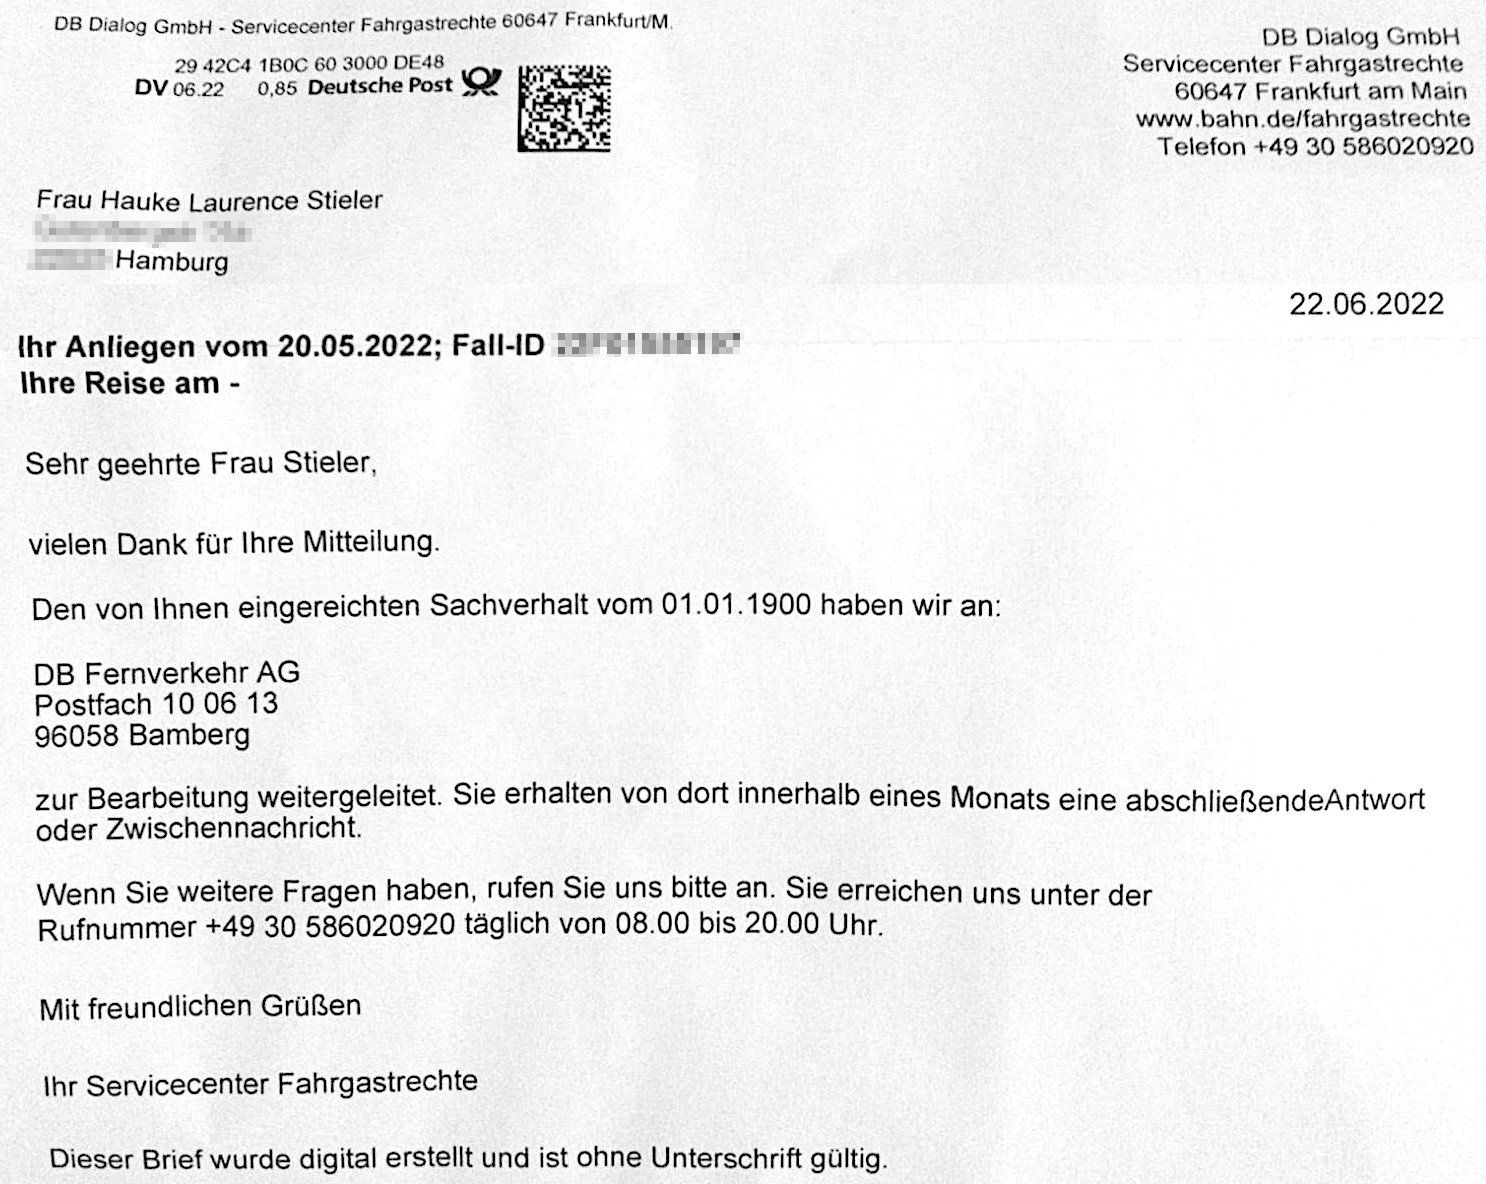
\includegraphics[width=\textwidth]{images/bahn-brief}};
			
			\only<2->{
				\draw[red,rounded corners=1mm] (4.75,4.375) rectangle (6,4.05);
			}
			
			\only<3->{
				\draw[red,rounded corners=1mm] (0.3,0) rectangle (3.5,0.325);
			}
			
			\only<4->{
				\draw[red,rounded corners=1mm] (1.8,7.85) rectangle (2.25,8.075);
			}
		
			\only<5->{
				\draw[red,rounded corners=1mm] (1.8,7.85) rectangle (2.25,8.075);
			}
		\end{tikzpicture}
	\end{frame}
	
	\begin{frame}[plain]
		\begin{tikzpicture}
   			\node[anchor=south west,inner sep=0] at (0,0) {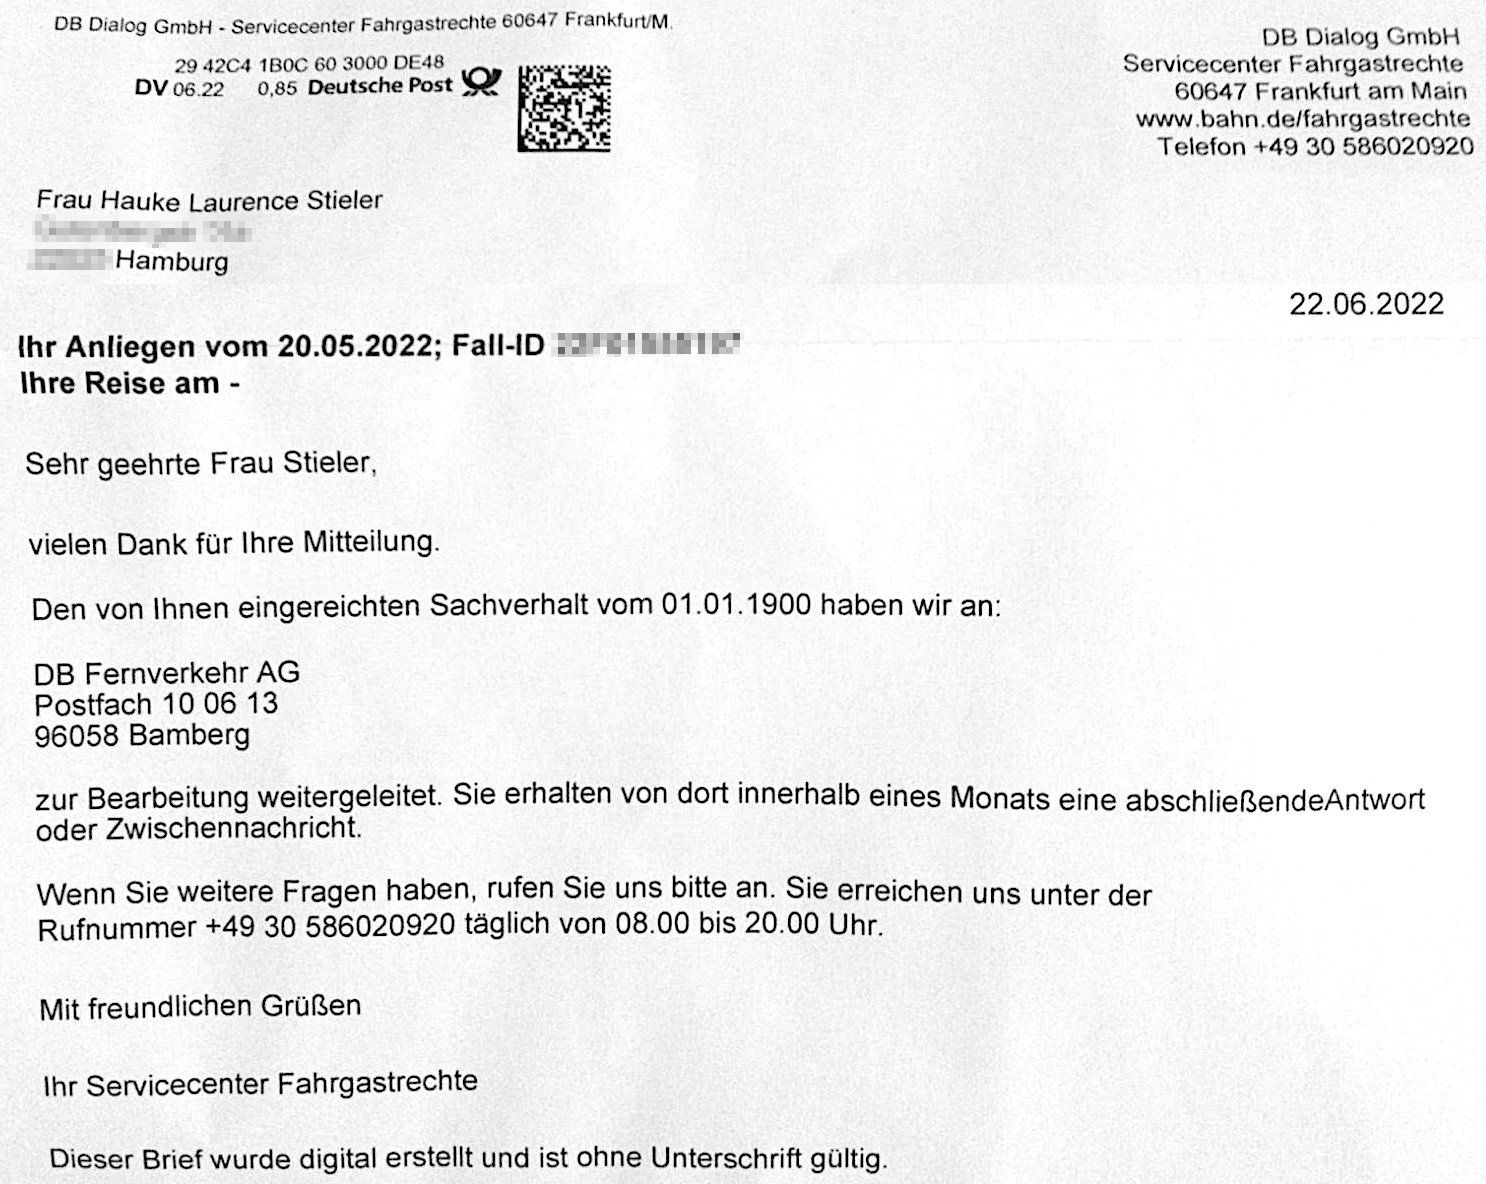
\includegraphics[width=\textwidth]{images/bahn-brief}};
   			
   			\only<2-4>{
			    \draw[red,rounded corners=1mm] (0.18,7.32) rectangle (0.75,7);
			    \draw[red,rounded corners=1mm] (1.45,5.4) rectangle (2.1,5.1);
   			}
   			\only<3-6>{
   				\node[anchor=west] at (4.9,6.7) {\small Bestätigung Kontaktformular:};
   				\node[inner sep=0.2mm,fill=black] at (6.5,5.275) {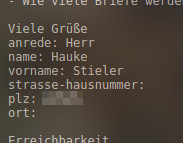
\includegraphics[width=3cm]{images/kontaktformular-bestaetigung}};
   			}
	   		\only<3-4>{
		   		\draw[red,rounded corners=1mm] (6,5.9) rectangle (6.65,5.65);
		   	}
   			\only<4-6>{
   				\node[anchor=west] at (4.9,3.7) {\small Antwort Kundendialog:};
   				\node[inner sep=0.2mm,fill=black] at (6.5,2.6) {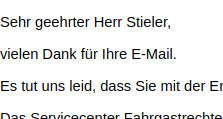
\includegraphics[width=3cm]{images/antwort-mail}};
   			}
	  		\only<4>{
		  		\draw[red,rounded corners=1mm] (6.2,3.25) rectangle (6.75,2.95);
		  	}
	   		\only<6>{
	   			\draw[red,rounded corners=1mm] (0.675,7.32) rectangle (2.85,7);
	   			\draw[red,rounded corners=1mm] (5.75,5.65) rectangle (7.05,5.15);
		   	}
		\end{tikzpicture}
	\end{frame}

	\begin{frame}[plain]
		\hspace*{-0.75cm}
		\vspace{-0.5cm}
		\begin{tikzpicture}[->,>=stealth']
			\draw[gray] (-1.5,4) -> (-0.5,4);
			\node[gray,anchor=west] at (-0.5,4) {Kommunikation};
			
			\draw[gray,dashed] (-1.5,3.5) -> (-0.5,3.5);
			\node[gray,anchor=west] at (-0.5,3.5) {Verwiesen an};
			
			\only<3-> {
				\draw[gray,densely dotted] (-1.5,3) -> (-0.5,3);
				\node[gray,anchor=west] at (-0.5,3) {Keine Ahnung};
			}
			
			\only<4-> {
				\draw[gray,dashdotted,-{Diamond}] (-1.5,2.5) -> (-0.5,2.5);
				\node[gray,anchor=west] at (-0.5,2.5) {Gehört zu};
			}
			
			\node (me) at (0,0) {Ich};
			
			\node (chatbot) at (4,3.5) {Chatbot\ \tiny(20.5.)};
			\draw (me) edge[<->] (chatbot);
			
			\node (chat) at (4.5,1.75) {Chat\ \tiny(20.5.)};
			\draw[dashed] (chatbot) -> (chat);
			
			\draw (me) edge[<->] (chat);
			
			\node (kontakt) at (4.75,0) {Kontaktformular\ \tiny(20.5.)};
			\draw[dashed] (chat) -> (kontakt);
			
			\draw (me) -> (kontakt);
			
			\node (db) at (4.5,-1.75) {Kundendialog\ \tiny(27.5.)};
			\draw (kontakt) -> (db);
			
			\draw (db) -> node[below] {\small Mail} (me);
			
			\node (fahrgastrechte) at (4,-3.5) {Fahrgastrechte\ \tiny(25.6.)};
			\draw (db) -> (fahrgastrechte);
			
			\visible<1-4> {
				\draw (fahrgastrechte) -> node[below left] {\small \textbf{Brief}} (me);
			}
		
			\visible<2-> {
				\node[align=center] (fernverkehr) at (8.5, 3) {DB Fernverkehr};
				\draw (fahrgastrechte) edge[out=10,in=205] (fernverkehr);
			}
		
			\visible<3-> {
				\node[align=center] (datenbank) at (8.5, -1) {Account-Daten};
			}
		
			\visible<4-> {
				\draw[densely dotted] (kontakt) edge[out=0,in=110] (datenbank);
				\draw[densely dotted] (db) edge[out=0,in=180] (datenbank);
				\draw (fahrgastrechte) edge[out=0,in=260] (datenbank);
			}
		
			\visible<6-> {
				\node (mensch) at (0.75,-3.5) {Mensch};
				\draw[dashdotted,-{Diamond}] (mensch) -> (fahrgastrechte);
			}
		
			\visible<7-> {
				\node (brief) at (-2,-2.5) {Brief};
				\draw (mensch) -> node[below] {\footnotesize 1. tippt} (brief);
			}
		
			\visible<8-> {
				\node (drucker) at (0.75,-1.75) {E-POST Treiber};
				\draw (mensch) -> node[right] {\footnotesize 2. drückt} (drucker);
			}
		
			\visible<9-> {
				\node (post) at (8,-4) {Post};
				\draw (fahrgastrechte) edge[out=270,in=180] node[below right] {\footnotesize 3. 0,85 €} (post);
			}
		
			\visible<10-> {
				\draw (brief) -> node[left] {\footnotesize 4. Post} (me);
			}
		\end{tikzpicture}
	\end{frame}

	\begin{frame}[plain]
		\vspace{-0.25cm}
		\begin{center}
			\hspace*{-1.2cm}
			
\includegraphics[width=1.2\textwidth]{images/conspiracy-meme}
		\end{center}
	\end{frame}

	\begin{frame}[plain]
		\vspace{-0.25cm}
		\begin{center}
			\hspace*{-1.2cm}
			
\includegraphics[width=1.2\textwidth]{images/digital erstellt}
		\end{center}
	\end{frame}

	\begin{frame}[plain]
		\begin{center}
			\vspace*{1cm}
			\hspace*{-1cm}
			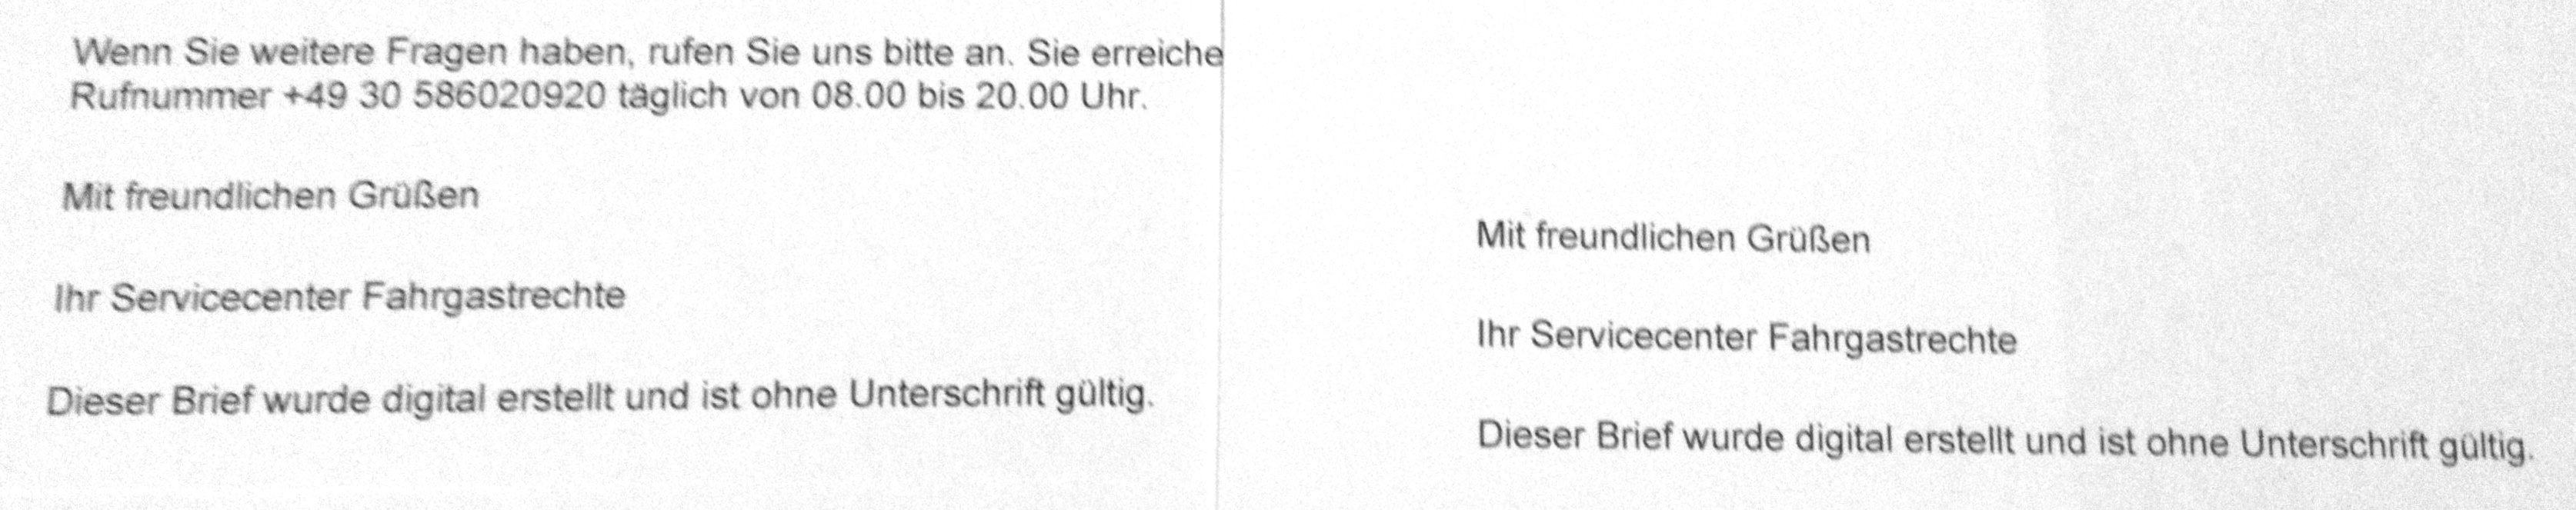
\includegraphics[width=1.15\textwidth]{images/bahn-brief-abschied}
		\end{center}
	\end{frame}

	\begin{frame}[plain]
		\begin{center}
			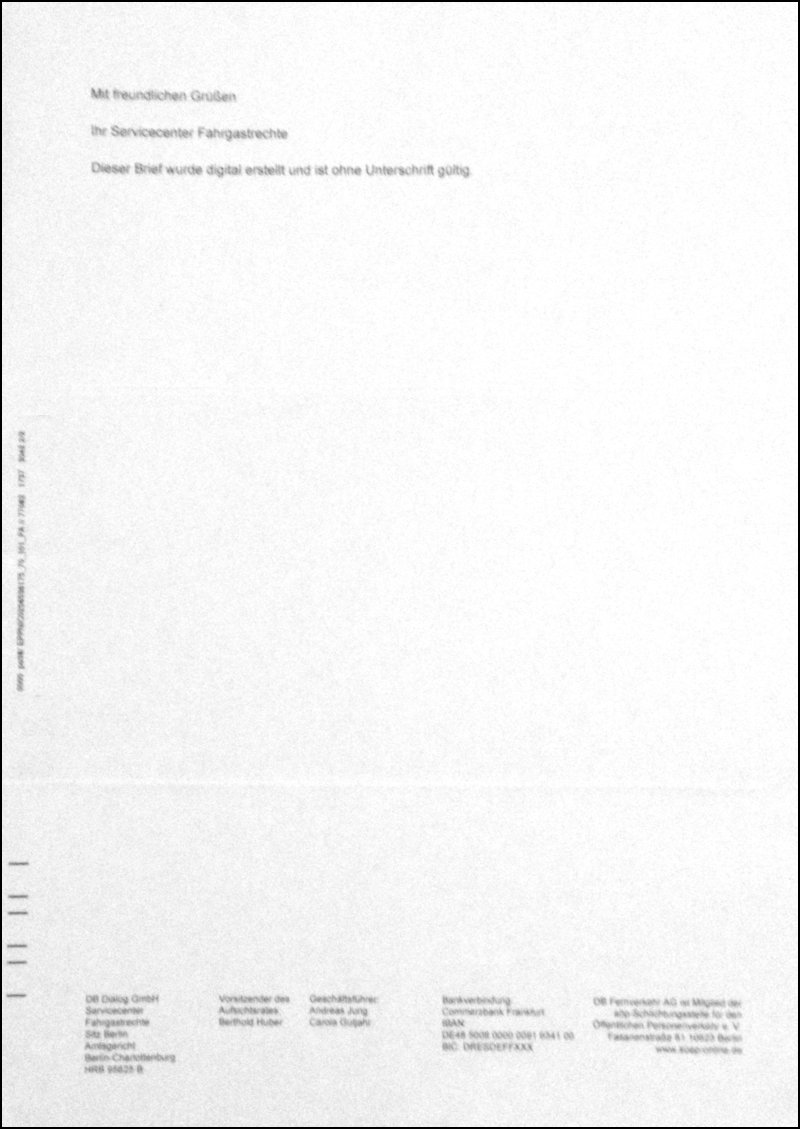
\includegraphics[height=1.2\textheight]{images/bahn-brief-page-2}
		\end{center}
	\end{frame}

	\begin{frame}[plain]
		\begin{tikzpicture}
			\node[anchor=south west,inner sep=0] at (0,0) {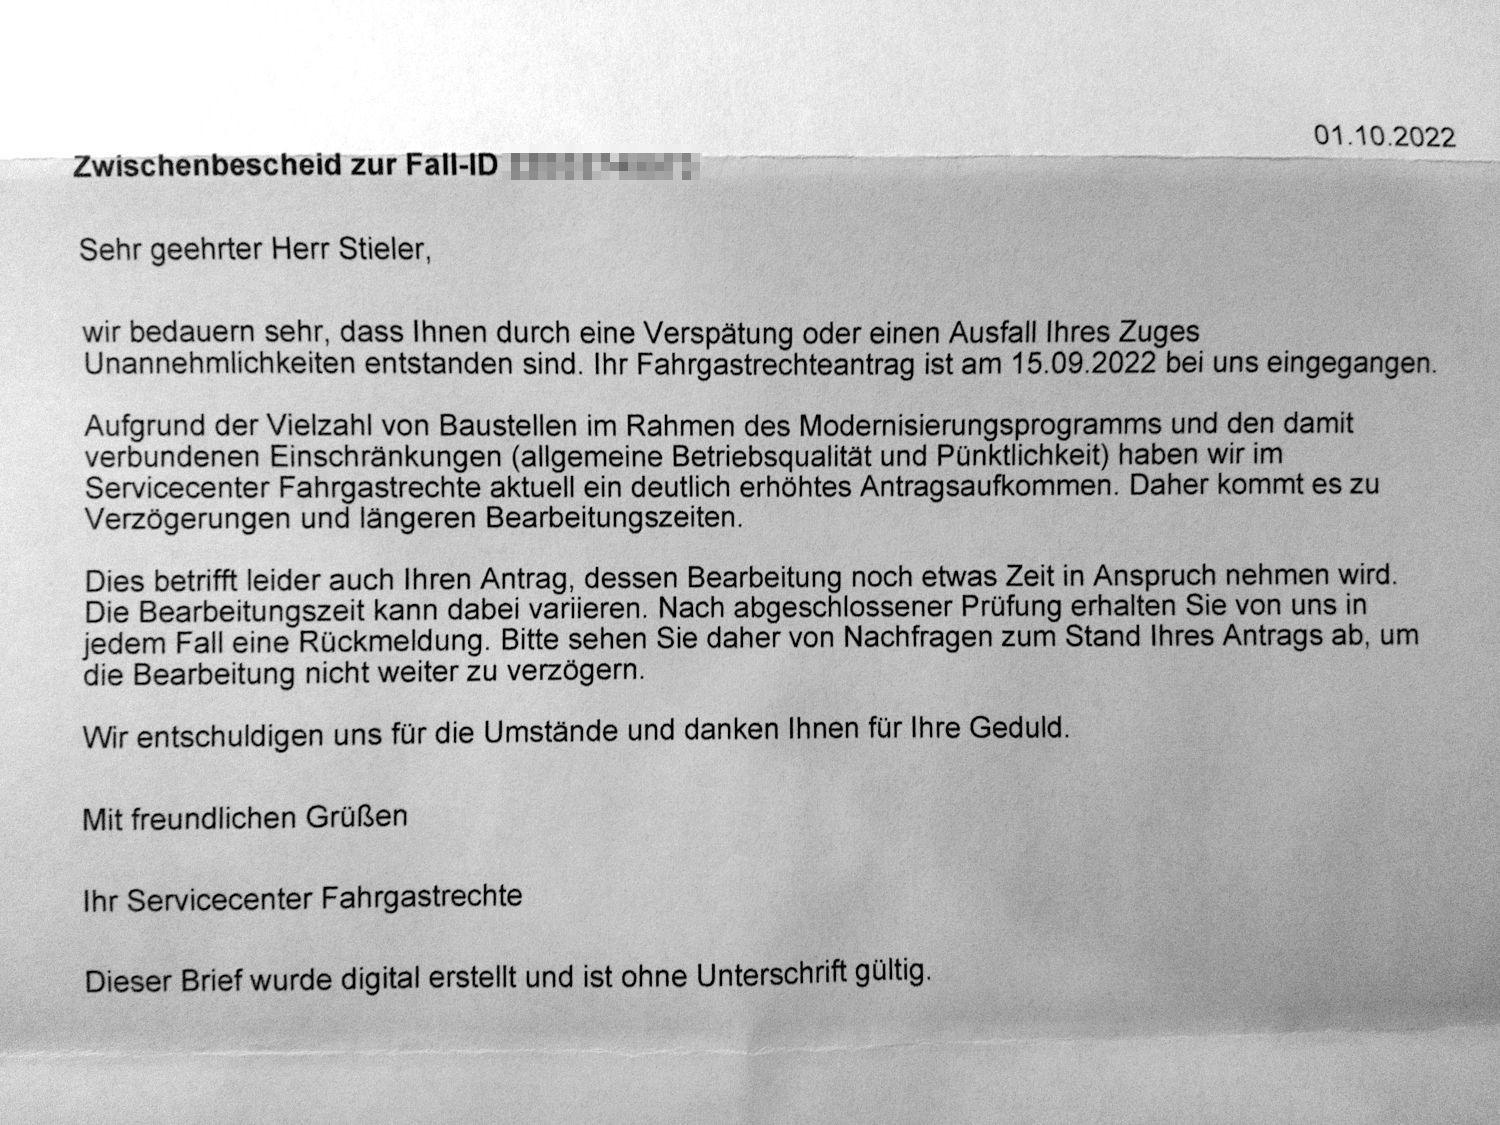
\includegraphics[width=\textwidth]{images/verzoegerung-briefe}};
			
			\only<1->{
				\draw[red,rounded corners=1mm] (7.68,3.6) rectangle (10,3.85);
				\draw[red,rounded corners=1mm] (0.55,3.32) rectangle (3.55,3.6);
			}
		\end{tikzpicture}
	\end{frame}

	\begin{frame}[plain]
		\begin{center}
			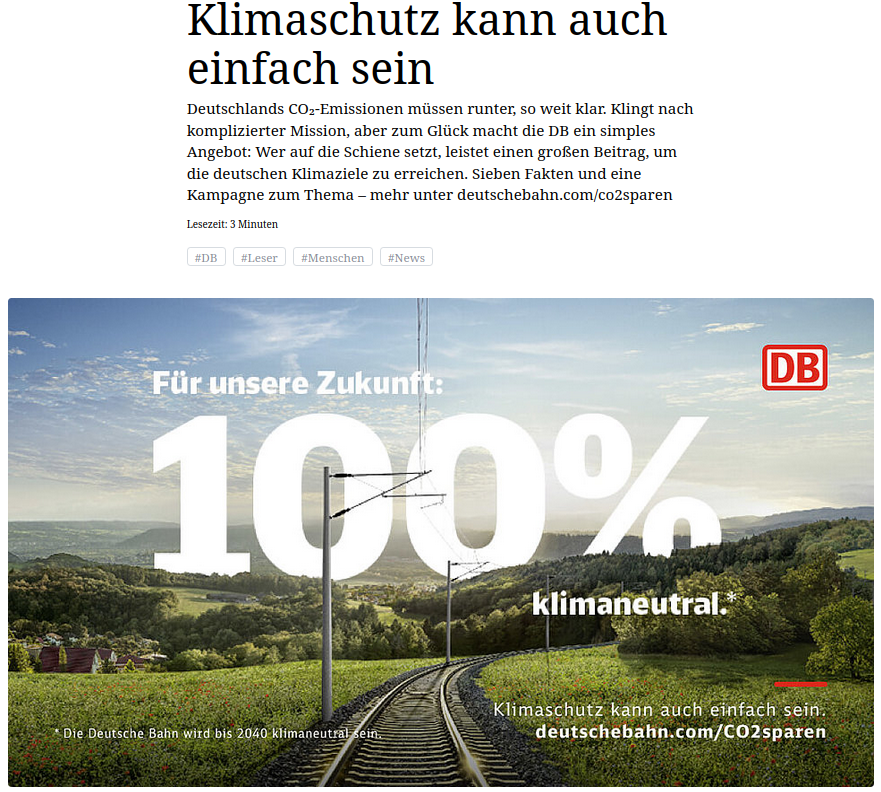
\includegraphics[height=1.2\textheight]{images/klimaschutz kann auch einfach sein}
		\end{center}
	\end{frame}

	\begin{frame}[plain]
		\begin{center}
			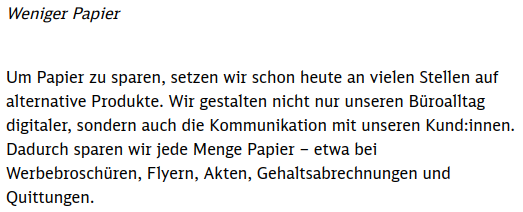
\includegraphics[height=0.5\textheight]{images/weniger papier}
		\end{center}
		\vspace{1cm}
		\scriptsize\url{https://gruen.deutschebahn.com/de/strategie/strategie-ressourcenschutz}
	\end{frame}
	
	\begin{frame}[plain]
		\begin{center}
			
\includegraphics[height=\textheight]{images/sceptical boy}\\
			\footnotesize(Hauke, Symbolbild)
		\end{center}
	\end{frame}

%	\begin{frame}[plain]
%		Laut  \href{https://www.tagesspiegel.de/wirtschaft/so-kommen-bahnkunden-am-schnellsten-an-eine-entschadigung-8019931.html}{tagesspiegel.de} für 2021:
%		\begin{itemize}
%			\item 1,9 Mio. Anträge\\\textrightarrow\ 5205 Anträge / Tag = 3,62 ApM\footnote{ApM = Anträge pro Minute}\\\textrightarrow\ ca. 4 Mio. Blatt Papier\\\textrightarrow\ 20t Papier
%			\item 38,2 Mio. \euro\ ausgezahlt \textrightarrow\ ca. 20€ pro Antrag
%		\end{itemize}
%	\end{frame}
%
%	\begin{frame}[plain]
%		\begin{itemize}
%			\item Portokosten = $0.85 \text{\euro} \cdot 1.9\text{ Mio.} = 1.6\text{ Mio. \euro}$\pause
%			\item Personalkosten / Brief = $5\text{ Min.} \cdot 25\text{ \euro\ Kosten\footnotemark} = 2.08\text{ \euro}$\\\textrightarrow\ Für alle Briefe: 4 Mio. \euro\pause
%%			\item Druckkosten = $0.02 \text{ \euro\ pro Blatt} \cdot 4 \text{ Mio.} = 100.000 \text{ \euro}$\pause
%%			\item Papierkosten = $0.01 \text{ \euro\ pro Blatt} \cdot 4 \text{ Mio.} = 40.000 \text{ \euro}$
%%			\item Kuvertkosten = $0.02 \text{ \euro\ pro Kuvert} \cdot 1.9 \text{ Mio.} = 38.000 \text{ \euro}$\pause
%		\end{itemize}
%		\vspace{0.5cm}
%		Kosten: 1.6M + 4M = 5.6M \euro\\
%		{\scriptsize (Zzgl. weitere Briefe, sonstige Ausgaben, Behörden- / Großkonzernfaktor, etc.)}
%		\footnotetext[2]{Kosten pro Stunde = Lohn nach \href{https://www.evg-online.org/fileadmin/Tarif/Tarifvertraege/weitere_Konzernunternehmen/DB_Dialog/21-08-23-DB_Dialog_ETV_01.03.2021-28.02.2023.pdf}{Tarif} $\times$ 2}
%	\end{frame}
%
%	\begin{frame}[plain]
%		\begin{center}
%			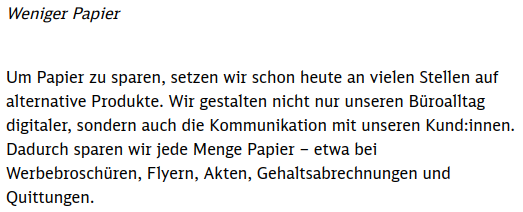
\includegraphics[height=0.5\textheight]{images/weniger papier}
%		\end{center}
%	\end{frame}
%
%	\begin{frame}[plain]
%		\begin{center}
%			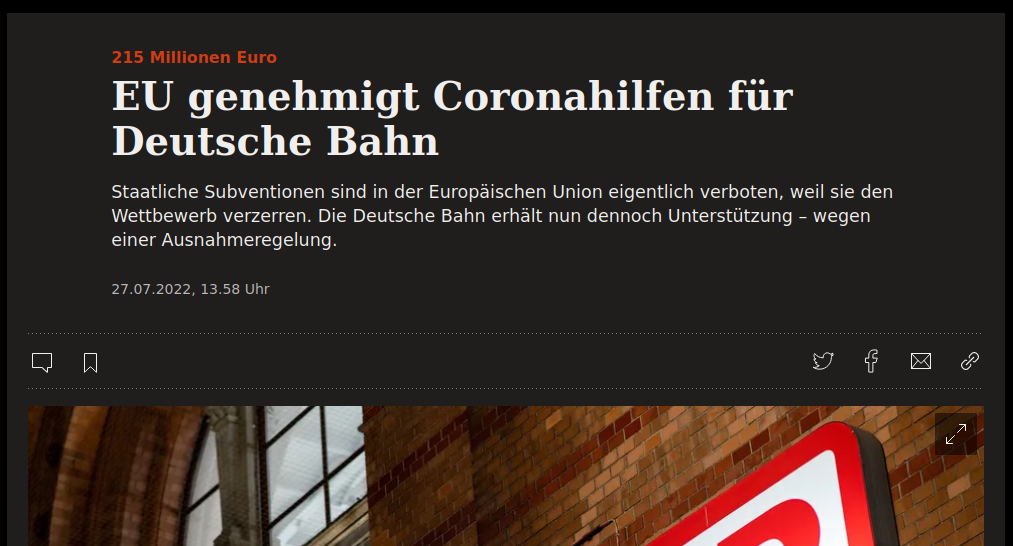
\includegraphics[width=\textwidth]{images/corona hilfen}
%		\end{center}
%	\end{frame}
%
%	\begin{frame}[plain]
%		\begin{center}
%			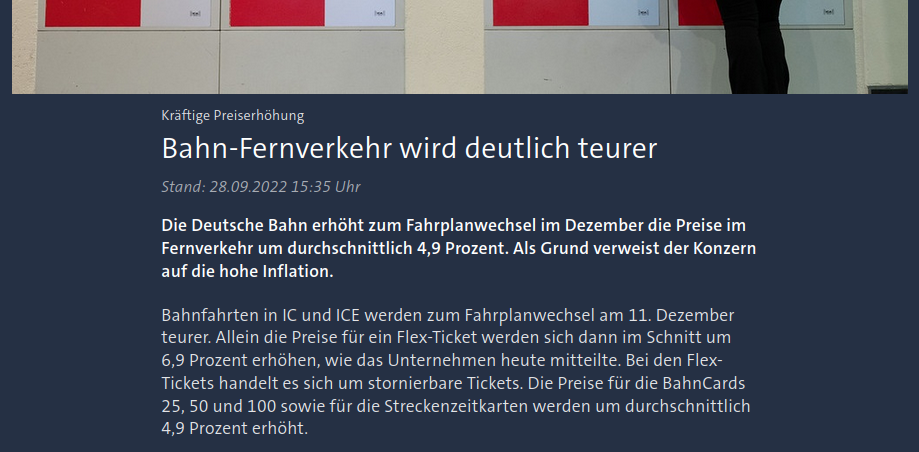
\includegraphics[width=\textwidth]{images/preiserhoehung}
%		\end{center}
%	\end{frame}
%
%	\begin{frame}[plain]
%		\vspace{0.5cm}
%		\begin{center}
%			
\includegraphics[width=0.7\textwidth]{images/bwl justus}
%		\end{center}
%	\end{frame}
%
%	\begin{frame}[plain]
%		\begin{center}
%			
\includegraphics[height=1.3\textheight]{images/bigger guy meme}
%		\end{center}
%	\end{frame}
\end{document}